\documentclass[journal]{IEEEtran}
\usepackage{cite}




 \usepackage[pdftex]{graphicx}



\begin{document}
\title{Effective Tumor Classification Exploiting Volumetric Image Analysis}
\author{Ashley J. Robinson}

% The paper headers
\markboth{Southampton University, Department of Electronics and Computer Science, Independent Research Review.}%
{Robinson: Effective Tumor Classification Exploiting Volumetric Image Analysis}

\maketitle


\begin{abstract}

This is what I gone done\dots

\end{abstract}







\begin{IEEEkeywords}
Tumor, Classification
\end{IEEEkeywords}



\IEEEpeerreviewmaketitle



\section{Introduction}
\IEEEPARstart{T}{his} research review covers the use of volumetric image analysis in medicine to accurately classify tumors. 
The problem is to be approached by considering only the general case where no specific area of the human body is considered.
Rather than trying to classify lung or brain tumors individually the goal is to consider what tumors have in common and given an entire image of a human body is it possible to classify tumors in any given section?
The motivation behind this is to make the most of medical scanning.
Dosages of radiation, cost and simply the time required are all reasons to reduce the number of scans needed, making the most of any data gathered is a constructive method of scan frequency reduction.
The objective is to provide a recommendation for a system to be implemented such that a medical practitioner could use it as a tool for diagnosis.  

The architecture in Figure~\ref{fig:Proposed} is a simplistic view of the system to be recommended; inspired by those discussed in ~\cite{ahmed2011efficacy,kumar2011classification,sachdeva2011multiclass}.
A chain of stages leads from raw data gathered from the patient to a diagnosis from a classification algorithm.
A confidence sub-block enables the domain expert to view the performance of the entire system without knowing the intricacies of operation; this requires processing to be explained with respect to their domain.

\begin{figure}[!htb]
   \centering
   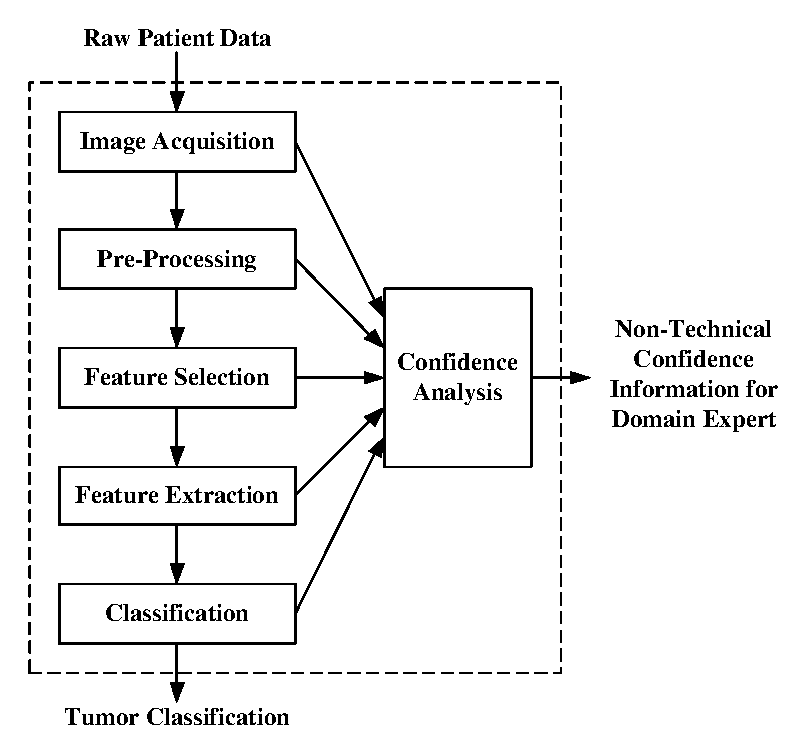
\includegraphics[width = 0.4\textwidth]{Figures/Proposed.pdf}
   \label{fig:Proposed}
   \caption{Proposed system architecture.}
\end{figure}



\section{Image Acquisition}
\label{sec:ImageAcquisition}
There are many pieces of medical equipment capable of extracting volumetric images of the human body using non-invasive techniques.
Most use CT technology to build an image from 2D slices.
These use X-ray, MRI and ultrasound technology to obtain the images, all of which have different trade offs between quality, health impact and efficiency~\cite{robb1999biomedical}.
Less well known techniques will also be investigated here such mechanical palpation~\cite{wellman1997modeling}. 




\section{Pre-processing}
\label{sec:PreProcessing}
How should the raw data outputted from the considered acquisition techniques be presented for further processing?
Depending on the equipment there may be a need to remove artifacts that were intended to assist visual inspection. 
Different types of 3D filters and the benefits they would bring will also be discussed.

\section{Feature Selection}
Here will be a sample of what type of features can be expected from the tumors.
Which are considered most important and which are known to be misleading.
A decision as to whether these can be rejected entirely from further processing can also be made. 

\section{Feature Extraction}
\label{FeatureExtraction}

The techniques used to extract the features.
This will make up a large amount of the report and will sample many different techniques and their objective performance~\cite{lohmann1998volumetric}.
The use of further dimensionality reduction will also be consider.


\section{Classification}
\label{Classification}

There are a many different classification algorithms available.
This section will consider expected data properties such as dimensionality and sparsity.
Availability of existing training data will constrain the application of supervised algorithms. 
The right classification algorithm can be recommended based on these findings.
Additional techniques, such as boosting, can also be considered.

\section{Conclusion}
\label{Conclusion}

This section will comment on how well the system can be pieced together.
A critical evaluation and discussion of all work done.


\bibliographystyle{ieeetran}
\bibliography{references}

\end{document}


